\documentclass[a4paper,10pt]{scrbook}
\usepackage{etex}
\usepackage[T1]{fontenc}
\usepackage{geometry}
\usepackage[utf8x]{inputenc}
\usepackage[ngerman]{babel}
\usepackage{graphics}
\usepackage{graphicx}
\usepackage{amssymb}
\usepackage{amsmath}
\usepackage{listings}
\usepackage{booktabs}
\usepackage{pdfpages}
\usepackage{pgfplots}
\usepackage{float}
\usepackage{latexsym}
\usepackage{longtable}
\usepackage{latexsym}
\usepackage{paralist}
\usepackage{enumitem}
\usepackage{pstricks}
\usepackage{stmaryrd}
\usepackage{MnSymbol}
\usepackage{array}
\usepackage{linearb}
\usepackage{titlesec}
\usepackage{listings}
\usepackage{xcolor}
\usepackage{xspace} 
\usepackage{hyperref} 
\usepackage{enumitem}

%Für Arrow listen
\newlist{arrowlist}{itemize}{1}
\setlist[arrowlist]{label=$\rightarrow$}


%Mehr Raum zwischen subsections
\titlespacing{\section}{0pt}{*4}{*2.5}
\titlespacing{\subsection}{0pt}{*3.5}{*1.5}

% kleine Anpassungen, damit die Seitenbreite überall außer Titel gleich ist.
\setcounter{secnumdepth}{2}
\setlength{\textwidth}{160mm}
\setlength{\textheight}{220mm}
\setlength{\headheight}{3mm}
\evensidemargin1mm
\oddsidemargin1mm

%Subsubsections werden hiermit nicht in das Inhaltsverzeichnis übernommen
\setcounter{tocdepth}{2}


%Dokumentenanfang mit diversen input von mehreren Einzeldokumenten.
\begin{document}
	\begin{titlepage}
\center
\Large Programmiersprachen\large \\[2em]
Lernskript \\[2em]
Dozent:\\Dr. Andreas Karwath\\[2em]
\LaTeX{} von:\\Sven Bamberger\\[2em]
Zuletzt Aktualisiert:\\\today\\

\includegraphics[scale=.2]{front/pics/Logo.jpg}\\\quad\\
\end{titlepage}
 
	
	\frontmatter 
		Dieses Skript wurde erstellt, um sich besser auf die Klausur vorzubereiten.\\
\qquad\\
\qquad\\
\textcolor{red}{\Large{Dieses Dokument garantiert weder Richtigkeit noch Vollständigkeit, da es aus Mitschriften und Vorlesungsfolien gefertigt wurde und dabei immer Fehler entstehen können. Falls ein Fehler enthalten ist, bitte melden oder selbst korrigieren und neu hoch laden.}}


		 
\tableofcontents 
 
	 
	\mainmatter 
	    \chapter{Haskell}
\label{sec:Haskell}
\section{Allgemein}
Haskell ist eine Funktionale Programmiersprache und ist daher um einiges anders als die bisher gelernten Objektorientierten Sprachen. Diese verwenden verstärkt funktionale Eigenschaften um sich weiter zu entwickeln. Funktionale Sprachen sind frei von Seiteneffekten und die Methoden können sich Gegenseitig nicht beeinflussen. Eine Methode liefert bei den gleichem Input immer den gleichen Output.
In diesem Dokument werden verstärkt Codebeispiele genutzt um die Sprache kurz zu erläutern. 
\section{Input, Main, Output}
Zunächst ein kleines "Hello World" Beispiel, wie es zu jeder Sprache gehört. Hier sieht man direkt wie die main von Haskell aufgebaut ist.
\newline
\begin{lstlisting}[language=Haskell]  
main = putStrLn "Hello World"
\end{lstlisting}
\qquad\newline
Um ein kleines Programm zu schreiben, was mehr tut, als lediglich Sachen auszugeben, müssen wir Input verarbeiten. Dafür ist Haskell nie wirklich vorgesehen worden, da dies unvorhergesehenes Verhalten erzeugen kann, welche Haskell vermeiden soll. Daher sollte man dies nur verwenden, wenn es gefordert oder nicht anders möglich ist. 
\newline
\begin{lstlisting}[language=Haskell]  
main = 	do
	print "What is your name?"
	name <- getLine
	print("Hello" ++ name ++ "!")
	-- main 
\end{lstlisting}
\qquad\newline
Wie man sieht, kann man den Input in eine vorher nicht definierte variable geben. In Haskell muss man variablen nicht vorher genauer definieren. Der Compiler versucht zur Compilezeit zu ermitteln, welchen Typ die Variable hat und setzt diesen fest. Wenn dies nicht möglich ist, wird die Variable zur Laufzeit erstellt und definiert und genau das kann zu unvorhergesehenem Verhalten führen. 
\subsection{IO}
IO Programme aus der Fragestunde, härter als das wird es aller Voraussicht nach nicht werden. 
\begin{lstlisting}[language=Haskell]  
putToConsoleAndCheck :: String -> IO Bool
putToConsoleAndCheck s = do
	if s == "" then return False 
	else do
	putStrLn s
	return True


putToConsoleAndReturnNothing :: String -> IO ()
putToConsoleAndReturnNothing s = do
	if s == "" then return () 
	else do
	putStrLn s
	return ()
\end{lstlisting}
\section{Funktionsdeklaration}
Eine Funktion in Haskell sieht ungewohnt aus und erinnert mich immer stark an Mathe. Wobei die späteren Listen Verarbeitungsmöglichkeiten noch stärker an die Mathematik angelehnt sind.
\newline
\begin{lstlisting}[language=Haskell]  
f :: Int -> Int -> Int
f x y = x*x + y*y
\end{lstlisting}
\qquad\newline
dies ist alles was genötigt wird um eine Funktion zu deklarieren. Vom Schreibaufwand ist dies sehr gering. Jedoch ist es ungewohnt eine Funktion so zu sehen. Also nehmen wir diese einmal komplett auseinander. 
\qquad\newline\qquad\newline
$\overbrace{f}^\text{Funktionsname} \underbrace{x \quad y}_\text{Variablennamen der Funktion} = \overbrace{x*x+y*y}^\text{was die Funktion macht}$
\qquad\newline\qquad\newline

Es sieht zwar nicht gerade überragend aus, jedoch ist hier schon sehr genau erklärt wie eine Funktion aufgebaut ist. 
$f :: Int -> Int -> Int$ ist die sogenannte Funktionstypendeklaration das erste $Int$ steht für das $x$ das zweite für $y$ und das dritte für den Typ des Ergebnisses. Es ist zwar nicht notwendig dies anzugeben, jedoch fördert es das Verständnis und hilft einem dabei nochmals genau über die Funktion nachzudenken. Da diese Methode jedoch auch gut für alle Zahlen geeignet ist, sollte man den Funktionstypen umdefinieren
\newline
\begin{lstlisting}[language=Haskell]  
f :: Num a => a -> a -> a 
\end{lstlisting}
\qquad\newline
Das sind nochmals kryptischer aus, jedoch bedeutet dies nur, dass die Funktion $f$ eine Zahl ($Num a =>"$) vom Typ $Num$ erwartet. Danach hätte es gerne noch eine Zahl und gibt eine Zahl zurück. Welche Typen diese Zahlen haben, wird zur Compilezeit definiert und entsprechend angewandt. Das $a->a->a$ bedeutet, dass alle vom Typ $Num$ sein müssen. Also wenn wir als erstes ein Int eingeben, werden alle $a$ zu einem Int und es werden nur noch Int's erwartet. Vorteil, wir können eine Funktion für unterschiedliche Zahlentypen verwenden, ohne diese jedes mal neu zu definieren. 

Auch können Funktionen weitere Funktionen aufrufen.
\newline
\begin{lstlisting}[language=Haskell]  
f :: Num a => a -> a -> a 
f x y = x*x + y*y

g :: Num a => a -> a -> a 
g = f 3
\end{lstlisting}
\qquad\newline

Wi funktioniert nun $g$? diese Funktion ruft nun $f$ mit dem Wert 3 auf und $f$ gibt sich die Funktion $f$ zurück um noch einen Wert entgegen zu nehmen. Dies bezeichnet man auch als Currying. 
Um zu verhindern, dass Haskell weiterhin die Typ Transformationen von Variablen übernimmt, kann man diese vorher definieren. Davon wird abgeraten, da dies zu unvorhergesehen Fehlern führen kann. z.B. wird der nach führende Code nie erfolgreich ausgeführt werden. 
\newline
\begin{lstlisting}[language=Haskell]  
x:: Int
x = 3

y:: Float
y=2,4

print (f x)
\end{lstlisting}
\qquad\newline

\section{Notation}
\subsection{Logik}

\begin{tabular}{cccc}
|| $\Rightarrow$ or 	& \&\& $\Rightarrow$ and  & ==  $\Rightarrow$ Gleichheit & /= $\Rightarrow$ Differenz  \\ 
\end{tabular} 

\subsection{Potenz}
\begin{tabular}{cc}
 x\^{}n & x**y \\  
\end{tabular} 

Hierbei gilt es zu beachten, dass n ein Int || Integer sein muss, und y irgend eine Variable vom Typ Num sein darf. 

\subsection{Listen}

\begin{itemize}
	\item sind getypt, es können lediglich Elemente eines Typs in einer Liste vorkommen (Mischen von Typen ist nicht möglich). Dies ergänzt sich mit Tupeln: Listen sind theoretisch beliebig lange Folgen von Elementen eines Typs, Tupel sind definiert lange Folgen von Elementen, die verschiedene Typen haben können. Typsignatur von Listen: z.B. [Int], [Char], usw.
	\item können polymorph sein, d.h., der Typ einer Liste kann parametrisiert werden. Typsignatur in diesem Fall: z.B. [a]
	\item können per Aufzählung der Elemente definiert werden (Beispiel: [1,2,3]) oder mittels des Listenkonstruktors (Beispiel: 1:(2:(3)) ).
	\item werden per Rekursion (x:xs beschreibt das erste Element x einer Liste und die Restliste xs) oder per Indizierung (Operator !!) verarbeitet (die Indizierung beginnt bei 0)
	\item können mittels Erzeugungsschemata beschrieben werden (list comprehensions): z.B. [ transform neueListe | neueListe <- alteListe, tollerTest neueListe ], in dem die Elemente einer existierenden Liste traversiert, optional mit Prädikaten gefiltert und ebenfalls optional durch weitere Funktionen transformiert in eine neue Liste übernommen werden. In diese Rubrik fällt auch eine abgekürzte Schreibweise für Aufzählungen: z.B. [1..10] um eine Liste mit Elementen von 1 bis 10 zu erzeugen.
	\item können dank Haskell´s Lazy Evaluation Strategie unendlich lang sein (ihrer Beschreibung nach), wie z.B. bei [1..]. Solche Listen können verwendet werden, solange für den gewünschten Zweck die Auswertung nur eines Teils der Liste ausreicht.
\end{itemize}

\subsubsection{Beispiele}
\begin{align*}
\text{[ ]} &\Leftrightarrow \text{leere Liste}\\
\text{[1,2,3]} &\Leftrightarrow \text{Liste von integralen}\\
\text{["foo","bar","baz"]} &\Leftrightarrow \text{Liste aus Strings}\\
\text{1:[2,3]} &\Leftrightarrow \text{[1,2,3] : ist das Symbol zum vorne anhängen an eine Liste}\\
\text{1:2:[ ]} &\Leftrightarrow \text{[1,2]}\\
\text{[1,2]++[3,4]} &\Leftrightarrow \text{[1,2,3,4] ++ ist für das konkatinieren zuständig}\\
\text{[1,2,3]++["foo"]} &\Leftrightarrow \text{Error, die Inahlte einer Liste müssen immer vom selben Typ sein.}\\
\text{[1..4]} &\Leftrightarrow \text{[1,2,3,4]}\\
\text{[1,3, .. 10]} &\Leftrightarrow \text{[1,3,5,7,9]}\\
\text{[2,3,5,7,11 ... 100]} &\Leftrightarrow \text{Haskell ist leider nicht so klug ;-) }\\
\text{[10,9 ..1]} &\Leftrightarrow \text{[10,9,8,7,6,5,4,3,2,1]}\\
\end{align*}

\subsection{Strings $\Rightarrow$ Liste aus Char}
'a' :: Char\\
\grqq  a\grqq   :: [Char]\\
\grqq  \grqq   $\Leftrightarrow$ []\\
\grqq  ab\grqq   $\Leftrightarrow$  ['a','b'] $\Leftrightarrow$  'a':\grqq  b\grqq   $\Leftrightarrow$ 'a':['b'] $\Leftrightarrow$  'a':'b':[]\\
\grqq  abc\grqq   $\Leftrightarrow$  \grqq  ab\grqq   ++ \grqq  c\grqq  

\subsection{Tupel}
Tupel können unterschiedliche Typen enthalten und beliebig groß sein, jedoch funktionieren die Standard Implementationen lediglich auf Tupel der Größe 2\\
\subsection{Beispiele}
\subsubsection{Tupelkonstruktionen}
(2,\grqq foo\grqq  ) Unterschiedliche Typen sind legitim in Tupel\\
(3,'a',[2,3]) Listen sind auch möglich in Tupel\\
((2,\grqq a\grqq),\grqq c\grqq ,3) Auch können Tupel in Tupel geschrieben werden\\
\subsubsection{Standardimplementationen}
fst(x,y) $\Rightarrow$ x \\
fst(x,y,z) $\Rightarrow$ Error, zu viele Elemente \\
snd(x,y) $\Rightarrow$ y\\
snd(x,y,z) $\Rightarrow$ Error, zu viele Elemente

\section{Currying}
Grundsätzlich sind alle Funktionen in Haskell curried. Curried bedeutet, dass die Funktion eine Funktion zurück liefert welche eine weitere Variable erwartet. 
\newline
\begin{lstlisting}[language=Haskell]  
f :: Num a => a -> a -> a 
f x  = x*x + y*y
\end{lstlisting}
\qquad\newline
Bei diesem Beispiel wird die Funktion mit $f$ 4 5 aufgerufen. Als erstes Ergebnis liefert die Funktion sich selbst zurück und nimmt die 5 als $y$ auf. Dadurch ist es möglich Funktionen kürzer zu gestalten. In den folgenden Beispielen als erstes die gecurriede Version und direkt im Anschluss die nicht gercurriede Version. 
\newline
\begin{lstlisting}[language=Haskell]  
Klassisches Currying
sum x y = x + y

Klassische ugecurriede Version
sum (x,y) = x + y
\end{lstlisting}
\qquad\newline
Auch lassen sich die Funktionen einfach Verkürzen. 
\begin{lstlisting}[language=Haskell]  
Ungecurriede Version
square :: Num a => a -> a
square x = x^2

Gecurriede Version
square :: Num a => a -> a
square' = (^2)
\end{lstlisting}
\section{if .. then .. else und Guards}
Hier einfach ein Beispiel der gleichen Funktion einmal mit if .. then .. else Konstrukt und einmal als Guards (diese erinnern mich immer sehr stark an Switches) welche auch mit Pattern Matching zusammenarbeiten. Bei einem if .. then .. else Konstrukt muss immer ein else Teil angegeben werden. Da der Compiler sonst streikt. Denn Funktionen sollen ohne Nebeneffekte ausgeführt werden können. Und ein Vergessenes else führt zu nicht vorhersagbaren Nebeneffekten. 
\begin{lstlisting}[language=Haskell]  
absolute :: (Ord a, Num a) => a -> a
absolute x = if x >= 0 then x else -x

absolute' :: (Ord a, Num a) => a -> a
absolute' x 
	| x >= 0 =x
	| otherwise = -x
\end{lstlisting}
\qquad\newline

\section{Typen und Typ Klassen}
\subsection{Standard Typen}
\qquad\\
\textbf{Int} ist ein ganzzahliger, an das System gebundener Wert. 32-Bit / 64-Bit\\ 
\textbf{Integer} ist auch ein ganzzahliger, nicht an das System gebundener Wert, es kann so groß werden, wie der Speicher groß ist. \\
\textbf{Float} eine echte Gleitkommazahl mit einfacher Genauigkeit. \\
\textbf{Double} eine echte Gleitkommazahl mit doppelter Genauigkeit. \\
\textbf{Bool} Boolean halt. \\
\textbf{Char} ein einzelnes Zeichen in Einfachen Anführungszeichen. 
\subsection{Standard Typ Klassen}\qquad\\
\textbf{Eq} 
\begin{lstlisting}[language=Haskell]  
(==) :: (Eq a) => a -> a -> Bool  
\end{lstlisting}\qquad\newline
\textbf{Ord} 
\begin{lstlisting}[language=Haskell]  
(>) :: (Ord a) => a -> a -> Bool  
\end{lstlisting}\qquad\newline
\textbf{Show} wandelt Zahlen und boolische Ausdrücke in Strings um\
\begin{lstlisting}[language=Haskell]  
show :: Show a => a -> String 
\end{lstlisting}\qquad\newline
\textbf{Read} wandelt Strings in Zahlen oder boolische Ausdrücke um. 
\begin{lstlisting}[language=Haskell]  
read :: (Read a) => String -> a  
\end{lstlisting}\qquad\newline
\textbf{Num} ist eine numerische Typ Klasse. Ihr Mitglieder lasen sich wie Zahlen benutzen und verhalten sich so.\\
\textbf{Enum} ist eine Typ Klasse, welche alle auf zählbaren / durchzunummerierende Sachen enthalten. dadurch lassen sich erst die unendlichen Listen darstellen. Auch können succ und pred als Funktionen auf dessen Mitglieder angewandt werden.  

\subsection{Eigene Typklassen}\qquad\\
\textbf{type Name = AnotherType}\\ Damit kann man dem Kind AnotherType einen neuen Namen geben. Wenn man z.B. zwischen Nachname und Vorname unterscheiden möchte. Jedoch macht der Compiler hier keinen Unterschied. \\\qquad\\
\textbf{data Name = NameConstructor AnotherType}\\ Hier macht der Compiler eine Unterscheidung. Der genaue Unterschied zwischen beiden type und data wird gleich an einem Beispiel erläutert.  \\\qquad\\
\textbf{data} \\ Damit kann man sich rekursive Strukturen definieren.\\\qquad\\
\textbf{deriving}\\ damit kann man sich Funktionen erzeugen lassen. 

\subsubsection{Beispiele}
Bei dem nachfolgenden Beispiel, muss man sehr aufpassen, denn die Type und Data Version haben starke Unterschiede zur Laufzeit. Wenn man die Type Version nutzt, kann man als Eingabe Color und Name vertauschen und das Programm arbeitet trotzdem weiter, da es lediglich Strings erwartet. \\
Bei Data erwartet Haskell wirklich Datenstrukturen Name und Color. Wenn man hier zuerst Color und danach Name eingibt, meckert der Compiler. 

\begin{lstlisting}[language=Haskell]  
Type Version
type Name   = String
type Color  = String

Data Version
data Name   = NameConstr String
data Color  = ColorConstr String

showInfos :: Name ->  Color -> String
showInfos (NameConstr name) (ColorConstr color) =
"Name: " ++ name ++ ", Color: " ++ color
\end{lstlisting}\qquad\newline
Als nächstes wird eine Rekursive Datenstruktur definiert und mit deriving(Show) erweitert, was dazu führt, das diese Datenstruktur direkt gedruckt werden kann. 
\begin{lstlisting}[language=Haskell]  
data Tree a = EmptyTree | Node a (Tree a) (Tree a) deriving (Show, Read, Eq)  
\end{lstlisting}
\section{Pattern Matching}\qquad\\
Beim Pattern Matching handelt es sich um die Möglichkeit in eine Funktion Abzweigungen einzubauen, aufgrund von bestimmten Inhalten einer Variable. Davon wird exzessiv in Prolog$^{\ref{sec:Prolog}}$ gebraucht gemacht. \\
Das Pattern Matching ist eine effiziente Art zu programmieren, wenn man wenige unterschiedliche Werte hat, auf die geprüft werden muss. Auch kann man damit gut Abbruchbedingungen erstellen für rekursive Funktionen. Dabei gilt zu beachten, dass von oben nach unten gearbeitet wird. 
\begin{lstlisting}[language=Haskell]
factorial :: (Integral a) => a -> a  
factorial 0 = 1  
factorial n = n * factorial (n - 1)  
\end{lstlisting}
\section{List Comprehension}
Mit List Comprehensions kann man einfach Listen nach zuvor definierten Regeln erstellen. Dies ist besonders nützlich, um viele Werte schnell zu generieren.
\subsection{Beispiele}
\begin{lstlisting}[language=Haskell]
[x^2|x<-[1..5]]
Ergebnis: [1,4,9,16,25] 
\end{lstlisting}
Der Bereich nach | ist der sogenannte Generatorbereich und wird dazu genutzt, die Regeln für das erstellen der einzelnen Variablen zu definieren. \\ 
\begin{lstlisting}[language=Haskell]
[(x,y)|x <- [1,2,3],y <- [4,5]]
Ergebnis: [(1,4),(1,5),(2,4),(2,5),(3,4),(3,5)] 
\end{lstlisting}
Man kann auch mehrere Variablen im Generator Bereich verwenden und dadurch eine Liste von Tupeln generieren wie im oberen Beispiel gezeigt.  Jedoch sollte man sehr auf die Reihenfolge der Generatoren achten, da diese das Ergebnis stark beeinflussen. \\
\begin{lstlisting}[language=Haskell]
[(x,y)|x <- [1,2,3],y <- [x..3]]
Ergebnis: [(1,1),(1,2),(1,3),(2,2),(2,3),(3,3)] 
\end{lstlisting}
Hier werden Dependant Generators verwendet. Die zu erzeugenden Werte für $y$ hängen von $x$ ab. Dadurch kann man sehr gut doppelte Werte vermeiden und andere Spielereien machen. \\

\section{Lambda ( $\lambda$ ) Funktionen}\qquad\\
Lambda Funktionen sind Namenlose Funktionen welche lediglich einmal verwendet werden. Dies macht es möglich Funktionen in Methoden zu definieren und hat unter anderem auch Einzug in Java gefunden. Lambda Funktionen werden mit einem $\backslash$ eingeleitet. Hier ein Beispiel für eine einfache Addition.\\
\begin{lstlisting}[language=Haskell]
(\x y -> x+y) 4 3
Ergebnis: 7
\end{lstlisting}\qquad\\
Auf diese Art und Weise kann man sich beliebige Funktionen überall einbauen. Wodurch besonders foldl und foldr stark werden. 
\section{Higher Order Functions}\qquad\\
Als Higher Order Functions werden Funktionen bezeichnet welche eine Funktion als erstes Argument entgegennehmen.
\textbf{map} \\
nimmt eine Funktion und eine Liste entgegen und verwendet diese Funktion auf jedes Element der Liste und generiert so eine neue. 
\begin{lstlisting}[language=Haskell]
map :: (a -> b) -> [a] -> [b]  
map _ [] = []  
map f (x:xs) = f x : map f xs  
\end{lstlisting}\qquad\\
\textbf{filter}\\
ist eine Funktion welche eine Funktion entgegen nimmt, welche einen booleschen Wert zurück gibt. z.B. even. Dazu nimmt es noch eine Liste auf. Das Ergebnis ist eine Lsite, welche zu die Übergebene Funktion mit true ergibt. 
\begin{lstlisting}[language=Haskell]
filter :: (a -> Bool) -> [a] -> [a]  
filter _ [] = []  
filter p (x:xs)   
| p x       = x : filter p xs  
| otherwise = filter p xs  
\end{lstlisting}\qquad\\
\textbf{foldl}\qquad\\
foldl wendet eine Funktion von \textbf{links} beginnend auf eine gesamte Liste an. \\
\begin{lstlisting}[language=Haskell]
foldl (\x y -> x^2 + y) 0 [1,2,3]
Ergebnis: 12
\end{lstlisting}\qquad\\
Was genau vor sich geht: \\
\begin{lstlisting}[language=Haskell]
foldl (\x y -> x^2 + y) 0 [1,2,3]
foldl (\x y -> x^2 + y) (0^2+1) [2,3]
foldl (\x y -> x^2 + y) (1^2+2) [3]
foldl (\x y -> x^2 + y) (3^2+3) []
foldl (\x y -> x^2 + y) 12 []
\end{lstlisting}\qquad\\
\newline
\textbf{foldr}\qquad\\
foldr wendet eine Funktion von \textbf{rechts} beginnend auf eine gesamte Liste an. \\
\begin{lstlisting}[language=Haskell]
foldr (\x y -> x^2 + y) 0 [1,2,3]
Ergebnis: 14
\end{lstlisting}\qquad\\
Was genau vor sich geht: \\
\begin{lstlisting}[language=Haskell]
foldr (\x y -> x^2 + y) 0 [1,2,3]
foldr (\x y -> x^2 + y) (3^2+0) [1,2]
foldr (\x y -> x^2 + y) (2^2+9) [1]
foldr (\x y -> x^2 + y) (1^2+13) []
foldr (\x y -> x^2 + y) 14 []
\end{lstlisting}

\section{Lazy Evaluation}\qquad\\
Haskell ist Faul! es berechnet nie das Ergebnis einer Funktion komplett sondern erst, wenn dies notwendig ist. Erst dadurch ist es möglich die Ranges zu verwenden um unendliche Listen zu erstellen. Es gibt zwei Methoden der Reduktion um Funktionen abzuarbeiten Innermost und Outermost. Haskell verwendet Outermost, da dies auch terminiert, sofern Innermost terminiert und es bleibt nicht in einer Endlosschleife hängen.  Jedoch ist Outermost Reduktion ineffizient und benötigt mehr Schritte. Um diesen Fehler zu umgehen benutzt Haskell Sharing. Dadurch wird es genauso effizient wie Innermost Reduktion und endet nicht in einer Endlosschleife.

\begin{figure}[h]
\centering
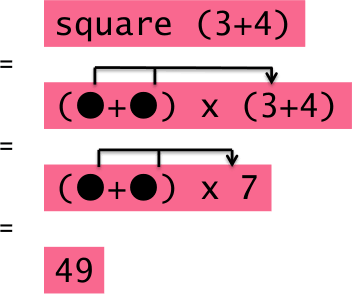
\includegraphics[width=0.25\linewidth]{mainmatter/pics/sharing}
\caption[Sharing + Outermost]{Sharing + Outermost}
\label{fig:sharing}
\end{figure}


  
  
	    \chapter{Prolog}
\label{sec:Prolog}
In Prolog dreht sich alles um das erstellen von Wissensbasen und deren Auswertung. Fakten und Regeln zusammen ergeben eine Wissensbasis und sind zusammen mit Anfragen die 3 Konstrukte aus denen sich diese Sprache zusammensetzt. Regeln und Fakten gehören und zu den Prädikaten. Fakten können weiterhin unterteilt werden in Funktoren und Atome. Dazu das passendes Bild. 

\begin{figure}[h]
\centering
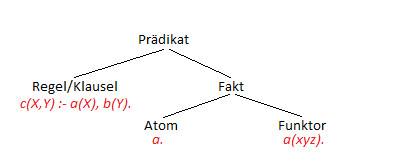
\includegraphics[width=0.5\linewidth]{mainmatter/pics/Prolog}
\caption[Prädikat Unterteilung]{Prädikat Unterteilung}
\label{fig:Prolog}
\end{figure}

\subsection{Atome}
\begin{itemize}
	\item fängt mit einem a-z
	\item bestehen aus den Zeichen a-z, A-Z, 0-9, \_
	\item Ein String in ' ' .z.B. 'Hi', auch als Name des Atoms bezeichnet. Leerzeichen sind innerhalb dieser Anführungszeichen erlaubt.
	\item Spezielle Zeichenketten sind erlaubt. Diese sind:
	\begin{enumerate}
		\item @= oder == oder ; oder :-  . Jedoch fallen ; und :- Sonderrollen zu. Mit ; fragt man nach weiteren Antworten von dem Programm und :- gehört fest zu einer Regel.
	\end{enumerate}
\end{itemize}
Hinweis: YAP und andere Prolog Interpreter erkennen 'mia' = mia. An und geben Yes aus. Jedoch '2' = 2. wird immer mit einem No konfrontiert. 
\subsection{Variablen}
\begin{itemize}
	\item Variablen beginnen mit A-Z oder \_ (mit \_ sind Anonyme Variablen) 
	\item bestehen aus den Zeichen a-z, A-Z, 0-9, \_
\end{itemize}\newpage
\section{Notation}
Im Nachfolgenden gibt es einen kleinen Überblick über die Notationen in Prolog.
\subsection{Und / Oder in Regeln}\qquad\\
, $\Leftrightarrow$ Und\\
; $\Leftrightarrow$ Oder
\subsection{Numerische Vergleichsoperatoren:}\qquad\\
\begin{align*}
\text{X }   &=:=  \text{  Y    numerisch gleich}\\
\text{X }  &=\backslash= \text{  Y    numerisch ungleich}\\
\text{X }   &<\text{   Y    X kleiner als Y}\\
\text{X }   &>\text{   Y    X größer als Y}\\
\text{X }  &=<\text{   Y    X kleiner gleich Y}\\
\text{X }  &>= \text{  Y    X größer gleich Y}\\
\end{align*}
!! Bei Vergleichen müssen alle Variablen belegt sein.



\subsection{Numerischer Auswertungsoperator:}\qquad\\
Ein einfaches Beispiel um X Berechnete Werte zu übergeben. \\
X is 6+3.\\
Achtung, wenn man X is Y + Z. schreibt, müssen Y und Z bereits belegt sein. Ansonsten führt dies zu einem Error. 

\subsection{Term-Vergleichsoperatoren:}\qquad\\
\begin{align*}
\text{X }   &=   \text{ Y    unifizierbar}\\
\text{X }  &\backslash=   \text{ Y    nicht unifizierbar}\\
\text{X }  &==   \text{ Y    identisch mit}\\
\text{X }  &\backslash== \text{ Y    nicht identisch mit}\\
\end{align*}




\subsection{Numerische Operatoren}

+     Addition

-     Subtraktion

*     Multiplikation

/     Division    

//    Ganzahl-Division

**    Potenz

mod   Modulo

/$\backslash$    bit-weises UND   (\& in C und C++)

$\backslash$/    bit-weises ODER  (| in C und C++)


\subsection{Typtest (nice to know but not necessary)}\qquad\\
Dies dient zur Bestimmung des Types der einzelnen Atome.\\
atom/1 	Is the argument an atom?\\
integer/1 	Is the argument an integer?\\
float/1 	Is the argument a floating point number?\\
number/1 	Is the argument an integer or a floating point number?\\
atomic/1 	Is the argument a constant? no var, or term. \\
var/1 	Is the argument an uninstantiated variable?\\
nonvar/1 	Is the argument an instantiated variable or another term that is not an un instantiated variable? \\
Dabei gilt besonders folgendes zu beachten bei dem Test auf atom. \\

\begin{lstlisting}[language=Prolog] 
Erst instanziert dann getestet. 
?-  X  =  a,  atom(X).
X  =  a
yes

Erst getestet dann instanziert. 
?-  atom(X),  X  =  a.
no 
\end{lstlisting}
\section{Wissensbasis}\qquad\\
Als Wissensbasis bezeichnet man eine Zusammenstellung von Fakten und Regeln. Im folgenden Beispiel ist alles vorhanden. 
\begin{lstlisting}[language=Prolog] 
happy(yolanda).
listens2Music(mia).
listens2Music(yolanda):-  happy(yolanda).
playsAirGuitar(X):-  listens2Music(X). 
\end{lstlisting}
Es gibt insgesamt 2 Fakten in dieser Wissensbasis. happy(yolanda) und listen2Music(mia). Diese Fakten werden auch Funktore genannt, da diese ein Atom einklammern. Ein Reiner Fakt würde z.B. yolanda sein. \\
Die letzten Beiden Zeilen in diesem Beispiel sind Regeln. diese Zeichnen sich durch :- aus und können auch Variable gehalten werden. Die erste Regel (listens2Music(yolanda):-  happy(yolanda).) wird per Pattern Matching (siehe dazu auch das Pattern Matching in Haskell$^{\ref{sec:hpm}}$) lediglich auf die Anfrage\\ ?-listen2Music(yolanda) reagieren. Alle anderen Fälle fängt die zweite Regel ab. Hier werden die Eingaben, mit X Unifiziert$^{\ref{sec:unifikation}}$. \\
Die Regel splittet sich in einen Kopf und einen Körper auf. Alles was vor dem :- steht ist der Kopf und alles was danach steht ist der Körper. 
\section{Rekursionen}\qquad\\
Auch in Prolog gibt es Rekursionen und diese werden stark genutzt. Damit können zum Beispiel Listen durchgearbeitet werden um zu schauen, wie lange eine Liste ist. Listen können hier beliebige Datentypen enthalten und sind nicht Typisiert wie in Haskell. 
\begin{lstlisting}[language=Prolog] 
len([],0) .
len([_|T],N):-len(T,X) ,N is X + 1.

Aufruf:
?- len([1,2,3,4],X).

Ergebnis:
X = 4?
yes
\end{lstlisting}
Nehmen wir diese Rekursion einmal auseinander.\\
Die erste Zeile in diesem Beispiel ist die Abbruch Bedingung. Diese wird wahr, wenn die Liste leer ist und definiert die Länge der leeren Liste als 0. Zu dieser 0 wird jeweils durch Backtracking, dem zurück schreiten im Lösungsbaum, eine eins hinzu addiert. Dies ergibt die Länge der Liste. \\
\qquad\\
Es ist \textbf{extrem wichtig}, dass die Abbruchbedingung als erste bei einer Rekursion genannt wird. Denn Prolog arbeitet von oben nach unten. Wenn wir zuerst die Rekursion (Zeile 2) geschrieben hätten würde dies zu einem Fehler führen. \\
Beginne bei einer Rekursion immer zuerst mit der Abbruchbedingung, und stelle den rekursiven Aufruf so weit wie möglich ans Ende der rekursiven Regel.
\section{Unifikation}\label{sec:unifikation}\qquad\\
Das Ergebnis einer Unifikation ist eine Liste von Variablenersetzungen, die man vornehmen muss, um zwei Ausdrücke identisch zu machen. Diese Liste ist Zustandsfrei (für alle Zeiten gleich und unveränderlich).\\ Prolog legt im Hintergrund jede Variable nach einem bestimmten Muster an. Dieses Muster ist \_5874 Wobei die Zahlen abweichen können. 
\begin{lstlisting}[language=Prolog] 
Beispiel 1:
eats(fred,tomatoes).
eats(Whom,What) .

Beispiel 2:
likes(jane,X).
likes(X,jim).

Beispiel 3:
f(foo,L).
f(A1,A1).

Beispiel 4:
X = t(X).
\end{lstlisting}\newpage
\textbf{Lösungen:}\qquad\\
\begin{enumerate}
	\item Unifikation ist möglich da Whom = fred und What = tomatoes. Bis hier hin keine große Verwunderung.
	\item Unifikation ist \textbf{nicht} möglich da X nicht gleichzeitig zwei Werten zugeordnet werden kann.
	\item Unifikation ist möglich. Denn A1 wird mit foo unifiziert und da L auch eine Variable ist, kann diese auch mit A1 und somit mit foo unifiziert werden. 
	\item Unifikation wird endlos weiter geführt. Denn X = t(X) = t(t(X)) \dots
\end{enumerate}
\section{Resolution}
\subsection{Was ist Resolution?}\qquad\\
Resolution ist die Vorgehensweise von PROLOG bei der Lösung von Anfragen.\\
Ob eine Zielanweisung zutrifft/erfüllbar ist wird durch den Widerspruch bewiesen. 
\subsection{Wie funktioniert Resolution ?}\qquad\\
Grundvoraussetzung für eine korrekte Arbeitsweise der Resolution ist eine Wissensbasis mit vollständigen, nicht widersprüchlichen Formeln. Da das Resolutionsverfahren korrekt ist wird es immer aus einer Formelmenge einen Widerspruch ableiten wenn sich darin einer befindet.\\
Die Anfrage an eine Wissensbasis ist nichts anderes als dass eine negierte Formel in die bereits vorhandene Menge gebracht wird. Trifft die Anfrage zu, so findet die Resolution einen Widerspruch und beweist somit deren Richtigkeit.\\
Dabei benutzt die Resolution das sogenannte Ableitungsverfahren. Dieses regelt das Zusammenfassen von Klauseln und geht dabei so vor:\\
Wenn der Kopf der 1.Klausel im Körper der 2.Klausel vorkommt, so kann an dieser Stelle der Körper der 1.Klausel eingesetzt werden.\\
\qquad\\
Zur Verdeutlichung:\\
1.Klausel: A :- B,C,D\\
2.Klausel: G :- E,F,A,K\\
ergibt\\
G :- E,F,B,C,D,K\\
\qquad\\
PROLOG geht dabei von oben nach unten vor, wenn mehrere vergleichbare Formeln vorhanden sind, so wird die \grqq oberste\grqq{} genommen, bei Nichterfolg wird die nächste versucht.\\
Sind mehrere Formel durch UND verknüpft, so wird dabei von links nach rechts vorgegangen, solange eine Beantwortung möglich ist. Bei verschiedenen möglichen Antworten wird immer die zuerst gefundene ausgegeben.
\newpage
\subsection{Ein Beispiel zur Vorgehensweise}\qquad\\
Gegebene Wissensbasis:\\
legs(X,2) :- mammal(X),arms(X,2).\\
legs(X,4) :- mammal(X), arms(X,0).\\
mammal(horse).\\
arms(horse,0).\\
\qquad\\
Stellt man nun die Anfrage:\\
?- legs(horse,4).\\
\qquad\\
geht PROLOG folgendermaßen vor:\\
diese Anfrage entspricht dem Kopf der 2. Regel, wenn man  nun X mit horse "unifiziert" und den Kopf durch den Körper der Regel ersetzt erhält man folgendes\\
:- mammal(horse), arms(horse,0).\\
nun wird mammal(horse)(da es ganz links steht kommt es zuerst dran) mit dem Fakt mammal(horse). aus der Wissenbasis 'gestrichen'.\\
Ebendies passiert auch mit dem arms(horse,0) welches nach der ersten "Streichung" geblieben ist und nun gestrichen wird.\\
Übrig bleibt die leere Klausel, d.h. der Widerspruch, womit die Zielanweisung als 'wahr' bewiesen wäre. 
\section{Akkumulatoren}\qquad\\
Akkumulatoren ist eine tolle Möglichkeit Variablen hoch zählen zu lassen, während eine Liste durchgegangen wird. Hier ein kleines Beispiel zur Berechnung der Länge einer Liste. \\
\begin{lstlisting}[language=Prolog] 
acclen([],A,A).
accLen([_|T],A,L):- Anew is A + 1, accLen(T,Anew,L).

Was passiert.
?-  accLen([a,b,c],0,L).
	Call:  (6)  accLen([a,  b,  c],  0,  _G449)  ?
	Call:  (7)  _G518  is  0+1  ?
	Exit:  (7)  1  is  0+1  ?
	Call:  (7)  accLen([b,  c],  1,  _G449)  ?
	Call:  (8)  _G521  is  1+1  ?
	Exit:  (8)  2  is  1+1  ?
	Call:  (8)  accLen([c],  2,  _G449)  ?
	Call:  (9)  _G524  is  2+1  ?
	Exit:  (9)  3  is  2+1  ?
	Call:  (9)  accLen([],  3,  _G449)  ?
	Exit:  (9)  accLen([],  3,  3)  ?
	Exit:  (8)  accLen([c],  2,  3)  ?
	Exit:  (7)  accLen([b,  c],  1,  3)  ?
	Exit:  (6)  accLen([a,  b,  c],  0,  3)  ? 
\end{lstlisting}
\newpage\qquad\\
Da der Rückgabewert nicht nochmal berechnet werden muss während des Backtrackings, sondern direkt bekannt ist, sind Akkumulatoren Programme effizienter als andere. \\
Besser erkenntlich wird dies wenn man sich folgendes Beispiel anschaut und durch den Kopf gehen lässt Mit hilfe des vorherigen Beispiels. \\
\begin{lstlisting}[language=Prolog] 
accRev([H|T],A,R):-accRev(T,[H|A],R).
accRev([],A,A).
rev(L,R):-accRev(L,[],R).
\end{lstlisting}
\section{Cut}\qquad\\
Das Prädikat Cut (Symbol !) wird verwendet, um unnötiges Backtracking zu verhindern. Der Cut ist stets erfolgreich.\\
\subsection{Wirkung:}\qquad\\
Wenn Prolog bei seiner Beweissuche den Cut (!) erreicht, dann können Entscheidungen links von dem Cut nicht mehr rückgängig gemacht werde.
\subsection{Arten:}\qquad\\
Ein grüner Cut schneidet Zweige des Suchbaumes ab, die keine Lösungen enthalten.\\
Ein roter Cut schneidet Zweige des Suchbaumes ab, die Lösungen enthalten. Diesen Cut sollte man vermeiden.
\subsection{Grüner Cut}
\begin{lstlisting}[language=Prolog] 
max(X,Y,Z) :- X =< Y, !, Z=Y.
max(X,_,X).
?- max(2,3,2).
No.
\end{lstlisting}
Es wird kein Backtracking mehr betreiben um weitere unnötige Lösungen zu finden. \\
Dies war z.B. Hilfreich um bei dem Affen Beispiel in der Vorlesung den Affen, nachdem er die Banane hatte nicht noch weiter im Raum herumlaufen zu lassen. \\
\newpage
\subsection{Roter Cut}
\begin{lstlisting}[language=Prolog] 
max(X,Y,Y) :- X =< Y, !.
max(X,_,X).
?- max(2,3,2).
Yes.
\end{lstlisting}
Hier ist die Lösung offensichtlich Falsch, denn 3 $\neq$ 2, jedoch wird daraufhin die zweite Regel angewandt, welche die Anfrage mit Yes beantwortet. Daher sind weitere Lösungsmöglichkeiten abgeschnitten.\\
$\Rightarrow$ roter Cut. 

\section{Zustände}\qquad\\
Zustände werden gentuzt um einen Weg (im besten Fall den kürzesten) zum Ziel zu beschreiben. Solche Zustände sind z.B. die Funktoren state bei der Monkey Aufgabe aus der Vorlesung. Anhand von diesen kann Prolog, mit Hilfe der Resolution, den Weg finden und das Ergebnis ausgeben. 
	    \chapter{C/C++}
\label{sec:C/C++}
In der Vorlesung wurde mehr C als C++ gelehrt und gezielt auf fortgeschrittenen Konzepte wie Klassen, Exceptions, Templates, etc. verzichtet. 
\section{Basics}
\subsection{Variablen}\qquad\\
\begin{itemize}
	\item fängt mir a-z oder \_ an.
	\item enthält a-z, A-Z, 0-9,\_
	\item darf \textbf{nicht} mit einer Zahl beginnen. 
	\item enthalten Werte eines festen Typs.
	\item muss deklariert werden, bevor diese verwendet werden kann. Am besten direkt mit einem Startwert deklarieren.
	\item nach Konventionen, muss die Variable mit einem kleinen Buchstaben beginnen. 
\end{itemize}
\subsection{Arithmetische Operatoren}
\begin{itemize}
	\item + Addition
	\item += Addition mit Zuweisung
	\item - Subtraktion
	\item -= Subtraktion mit Zuweisung
	\item * Multiplikation
	\item *= Multiplikation mit Zuweisung
	\item / Division
	\item /= Division mit Zuweisung
	\item \% Modulo
\end{itemize}
\subsection{Increment / Decrement}
\begin{tabular}{ccc}
	& prefix & postfix \\ 
increment	& ++a & a++  \\ 
decrement	& --a & a-- \\ 
\end{tabular} \\\qquad \\
Der Unterschied zwischen prefix und postfix ist, dass bei einer Zuweisung wie
\begin{lstlisting}[language=C++] 
a = ++b;
\end{lstlisting}
der Wert von b erst erhöht wird und danach erst zugewiesen wird. Bei 
\begin{lstlisting}[language=C++] 
a = b++;
\end{lstlisting}
wird der Wert erst zugewiesen und daraufhin erhöht. 
\subsection{Typen}
\begin{figure}[h]
\centering

\includegraphics[width=0.75\linewidth]{mainmatter/pics/typ}
\caption[typen]{Alle Typen im Überblick}
\label{fig:typ}
\end{figure}
Jedoch gilt es zu beachten das long und int meist gleich lang sind auf 32Bit Systemen und das der C++ Standard lediglich die Minimale Größe Garantiert.
\subsection{Logik Operationen}\qquad\\
\&\& / and = Und\\
|| / or = Oder\\
! / not = Negation\\
0 = false\\
alles $\neq$ 0 = true
\subsection{Vergleiche}
== ; < ; > ; >=; <= ; !=
		
\subsection{Funktionen}
\begin{lstlisting}[language=C++]
return_type name (parameters) {
	//body
}
\end{lstlisting}
Die Main Funktion wird mit dem return\_type int versehen, da Programme in der Regel eine 0 zurückliefern, sofern diese ohne Probleme durchgelaufen sind. 
\section{Programme Kompilieren}
\subsection{C++ Programme bauen}\qquad\\
Ein Programm in C++ kann aus mehreren Header Dateien (*.h) und Quellcode Dateien (*.cpp) bestehen. Um diese zu einem Lauffähigen Programm umzuwandeln. Benötigt man einen Compiler wie g++. Dieser Besteht aus einem Linker, Preprocessor und dem Compiler selbst. \\
Der Preprocessor nimmt alle in den Sourcecode verlinkten Header Dateien und fügt diese zu 100 \% in den Sourcecode in dieser Stelle ein. Die Header Dateien können gleichzeitig in mehreren Sourcecode Dateien stecken. \\
Der Compiler wandelt anschließen die Sourcecode Dateien in Objectdateien um, welche vom Menschen nciht mehr gelesen werden können.\\
Der Linker fügt alle Object Dateien mit den verwendeten externen Bibiliotheken zu einem ausführbaren Programm zusammen. Dabei werden auch alle Sprungadressen für Funktionsaufrufe gesetzt\\
\begin{figure}[h]
\centering
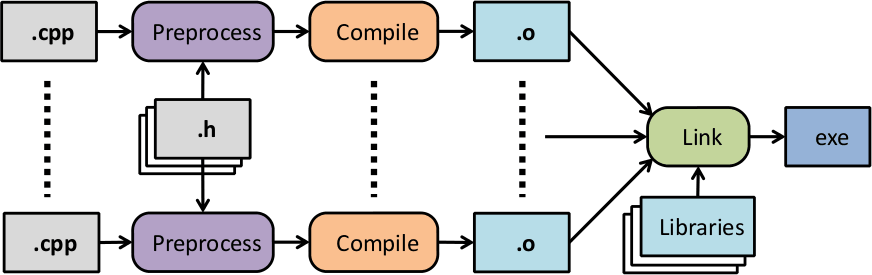
\includegraphics[width=0.75\linewidth]{mainmatter/pics/comp}
\caption[compiling]{C++ Programm Kompilieren}
\label{fig:comp}
\end{figure}
\subsubsection{Wozu dieses große Konstrukt?}
Viele Projekte enthalten eine sehr große Menge an Quellcode Dateien. Da man nicht bei jeder kleinen Änderung alle cpp Dateien neu in Objekt Dateien umwandeln will. Kann man auch schlicht nur die geänderten cpp Dateien durch den Preproccesor jagen und anschließend alle .o Dateien neu zu verlinken um die Änderungen zu testen. \\
Außerdem können vorhandene doppelte \#includes verhindert werden, indem man diese mit Guards definiert. Diese verhindern, dass die header Dateien, selbst bei mehrfacher Verlinkung, mehrfach in den Code einkopiert werden. \newpage
\begin{lstlisting}[language=C++]  
//Datei: foo.h
#ifndef A_H
#define A_H
struct foo {
	int member;
};
void f(foo&);
...
#endif
\end{lstlisting}
Selbst wenn man nun die foo.h header Datei in mehreren Dateien included, wird sie lediglich einmal hinzugefügt. Denn der Preprocessor, erkennt alle mit \# markierte Zeilen als seine an und führt das if entsprechend der Definition aus. Dabei geht der Guard von \#ifndef A\_H bis \#endif. Das \#define bedeutet, wenn A\_H noch nicht definiert wurde, definiere diese wie folgt. \\
\subsection{Wie lauten die Terminal Befehle dafür?} 
Die Terminal Befehle lauten wie folgt. 
\begin{lstlisting}[language=bash]
g++ -c source.cpp 
g++ -c dbl.cpp 
g++ source.o dbl.o -o test 
\end{lstlisting}
Mit dem Parameter -c werden die angegebenen cpp Dateien in Object Files umgewandelt. Danach linkt man die Object Files mit Hilfe des Parameters -o. Man kann auch direkt -o verwenden wenn man die Dateien direkt in eine .exe Datei umwandeln will.\\
Um das Kompilieren zu vereinfachen, benutzt man bei vielen Dateien eine Makefile. Einen solche sieht wir folgt aus. 
\begin{lstlisting}[language=bash]
#name test
#comment
#compile main 
main.o : main.cpp 
	g++ -c main.cpp 
#compile other 
other.o : other.cpp 
	g++ -c other.cpp 
#link 
prog: main.o other.o 
	g++ main.o other.o -o prog 
\end{lstlisting}
Der Aufruf der Makefile läuft folgendermaßen
\begin{lstlisting}[language=bash]
make test
./prog 
\end{lstlisting}
Mit ./ führt man die generierte .exe aus. 
\section{Kommandozeilen Argumente}
Hier ein kleines Beispiel, wie man Kommandozeilen Argumente beim Start eines Programmes direkt übergibt, ausliest und auf der Konsole ausgibt. 
\begin{lstlisting}[language=C++]
#include <iostream>

using namespace standard

int main(int argc, char* argv[])
{
for(int i = 1; i<argc;++i){
cout << argv[i] <<endl;
}
return 0;
}
\end{lstlisting}
\begin{lstlisting}[language=Bash]
> ./test 12 3 abc def
test
12
3
abc
def
\end{lstlisting}
argc und argv sind nur Konventionen und können anders benannt sein. argc enthält die Anzahl der Elemente und argv ist ein C Array. Die Elemente von argv sind wiederum C Strings.  
\section{I/O from console/file}	\qquad\\

\section{Control Statements and Loops}
\subsection{if .. then .. else / Switch}
\begin{lstlisting}[language=C++]
if (condition1) {
	//do this if condition1 is true
}
else if (condition2) {
	//otherwise do this if
	//condition2 is true
}
else {
	//otherwise do this 
}
\end{lstlisting}
\qquad\\
\begin{lstlisting}[language = C++]
switch(m){
	case 0:
		//do this if 0
		break;
	case 1:
		//do this if 1 and got to the next 
		//cause of missing break
	case 3: 
		//do this if 3
	break;
	default:
		// if everything else fails do this	
}
\end{lstlisting}
Für das m im switch können char, int, long und weitere Zahlenwerte verwendet werden. 

\subsection{Loops}
\begin{lstlisting}[language=C++]
for (int i = 0; i < 5; ++i) {
cout << i << endl;
}

int j = 5;
while (j < 10) {
cout << j << endl;
++j;
}

do {
cout << j << endl;
--j;
} while (j > 0);
\end{lstlisting}	
\section{Call by Value / Call by Reference}
\section{Pointer und Referenzen}
\subsection{Referenzen}
Referenzen referenzieren einen Wert lediglich. Wenn man den Wert einer Referenz ändert, so ändert man den Wert der Variable auf den die Referenz zeigt. Dies ist nützliche, da man Werte als Referenzen an eine Methode übergeben kann. Dadurch hat man die Möglichkeit sich mehr als einen return Wert zu generieren. Da man die Variable außerhalb der Methode ändert und nicht nur die Unbekannte innerhalb der Methode. \\
\begin{lstlisting}[language=C++]
// Initialisierung
int i = 2;
int& ri = i; 
const int& ci = i;
double& blub = i; // => Fehler da die Typen identisch sein muessen.
int& rj; // Fehler, da Referenzen immer initialisiert sein muessen

// Wertzuweisung

\end{lstlisting}
\section{Memmory Management (Stack/Freestore)}
\section{Structs}
\section{Complex Data Structures (Lists, Trees)}
\section{Standard Containers and Algorithms}	


	\backmatter
		\listoffigures 
\end {document}
